\documentclass[titlepage,10pt,a4paper]{article}
\usepackage[utf8]{inputenc}
\usepackage{graphicx}
\usepackage{hyperref}
\usepackage[ngerman]{babel}
\usepackage{float}
\usepackage{subcaption}
\usepackage{listings}
\usepackage{color}

\title{Handbuch}
\date{\today{}, Passau}

\begin{document}
\begin{titlepage}
\vspace*{3cm}
\begin{center}
\textbf{\textsc{\LARGE Handbuch}}

{\large \today}

\vspace{2cm}
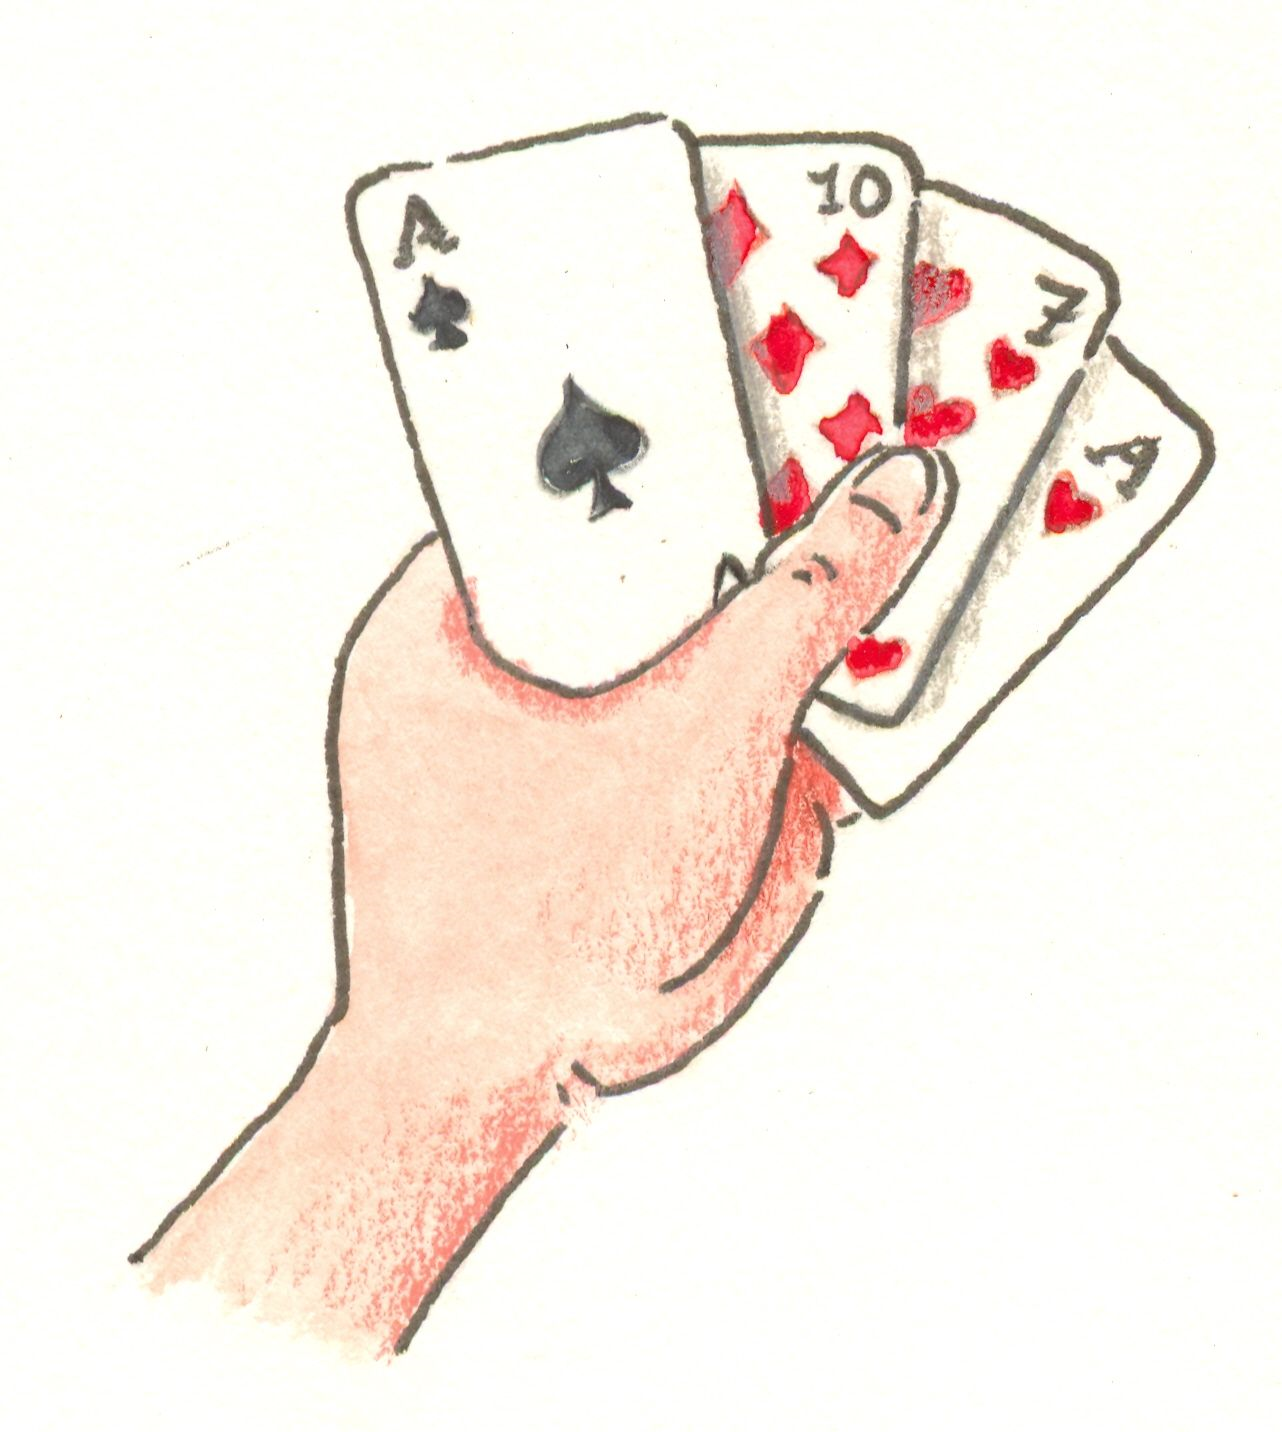
\includegraphics{kartenspiel}
\ \\
\ \\

\textbf{\textsc{\LARGE NET-WizHearts}}
\vspace{2cm}

\begin{tabular}{|c|c|c|}\hline
   Phase & Verantwortlicher & E-Mail \\ \hline\hline
   Pflichtenheft & Alina Meixl &  alina@meixl.de \\ \hline
   Entwurf & Viktoria Witka & witkaviktoria@freenet.de \\ \hline
   Spezifikation & Daniel Riedl & dariedl14@yahoo.de \\ \hline
   Implementation & Andreas Altenbuchner& a.andi007@gmail.com\\ \hline
   Verifikation & Patrick Kubin & kubin@fim.uni-passau.de\\ \hline
   Präsentation & w& w\\ \hline
 \end{tabular}
\vspace{2cm}
\\
\end{center}
\end{titlepage}
\tableofcontents
\pagenumbering{arabic}
\hypersetup{pageanchor=true}

\newpage
 
\section{Einleitung}
Dies ist das Handbuch zum Spiel NET-WizHearts. NET-WizHearts ist eine Plattform auf der mehrere Spieler online gegeneinander spielen können. Es gibt verschiedene Regelwerke, die gespielt werden können. Mitgeliefert werden bereits Hearts und Wizard. Die Plattform ist so konzipiert, dass jederzeit weitere Regelwerke hinzugefügt werden können.

\section{Installation}

\section{Spiel}
\subsection{Einloggen}
Loggen Sie sich zunächst in diesem Fenster ein.
\subsection{Spiel betreten}
In der Spiellobby können Sie einem existierenden Spiel beitreten.
\subsection{Spiel erstellen}
In der Spiellobby können Sie ein neues Spiel erstellen.
\subsection{Spiel spielen}
Das Spiel wurde gestartet, Sie befinden sich nun im Spielfenster.
\subsubsection{Wizard}
\subsubsection{Hearts}

 
\section{Glossar}

\end{document}